\chapter{Comparison with QUIJOTE-MFI Data}\label{ch:comparison_quijote}

\section{Comparison with Raw Data}

\begin{figure}
        \centering
        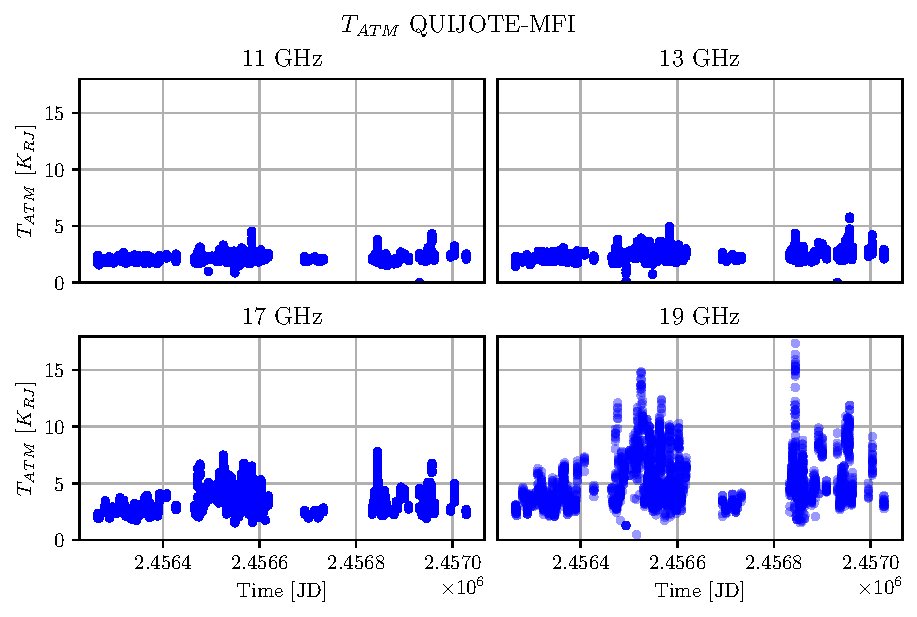
\includegraphics[width=\textwidth]{QUIJOTE_Dataset}
        \caption{QUIJOTE-MFI  $T_{atm}$ dataset.}
        \label{fig:quijote_dataset}
\end{figure}

\begin{figure}
        \centering
        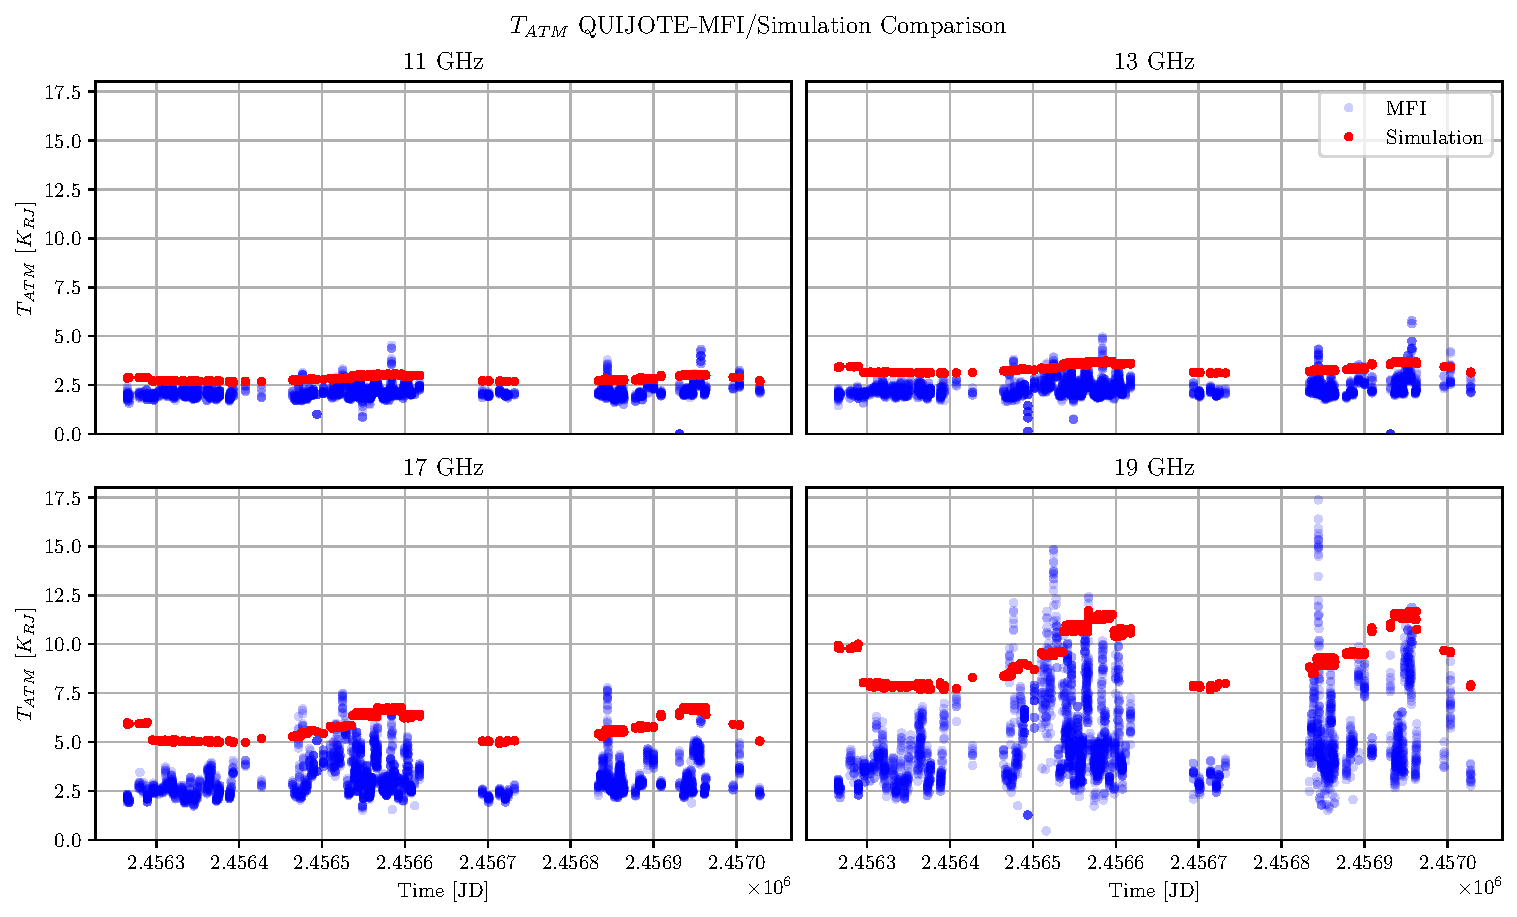
\includegraphics[width=\textwidth]{QUIJOTE-Sim}
        \caption{Comparison between QUIJOTE-MFI measurements and CAL
        simulated data.}
        \label{fig:quijote_sim}
\end{figure}

\section{The Calibration Coefficient}

\begin{figure}
        \centering
        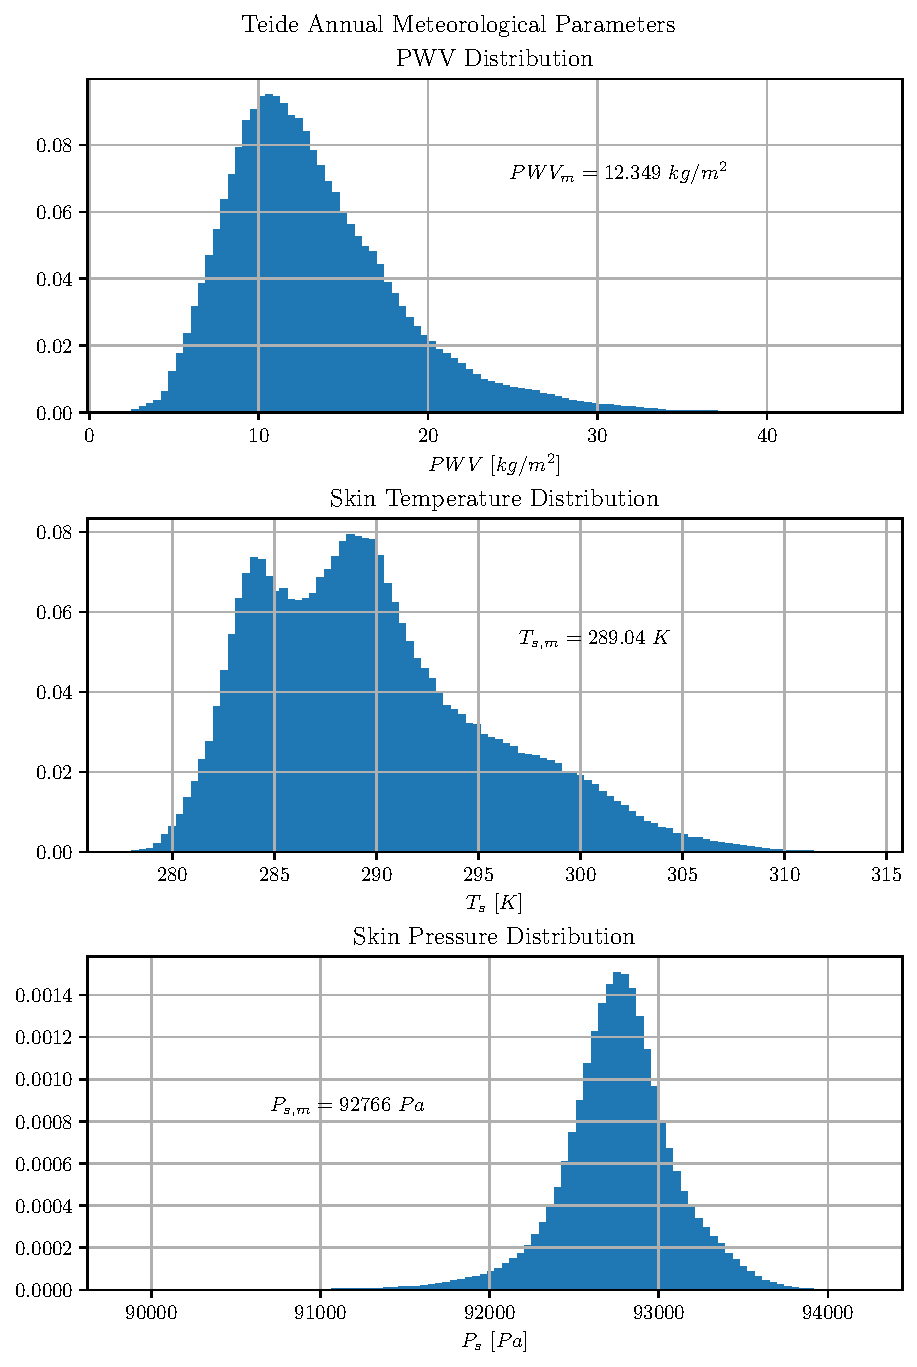
\includegraphics[width=0.93\textwidth]{Teide_Annual_Distributions}
        \caption{Annual distribution for relevant meteorological parameters
        at Pico del Teide.}
        \label{fig:teide_annual_distributions}
\end{figure}

\begin{figure}
        \centering
        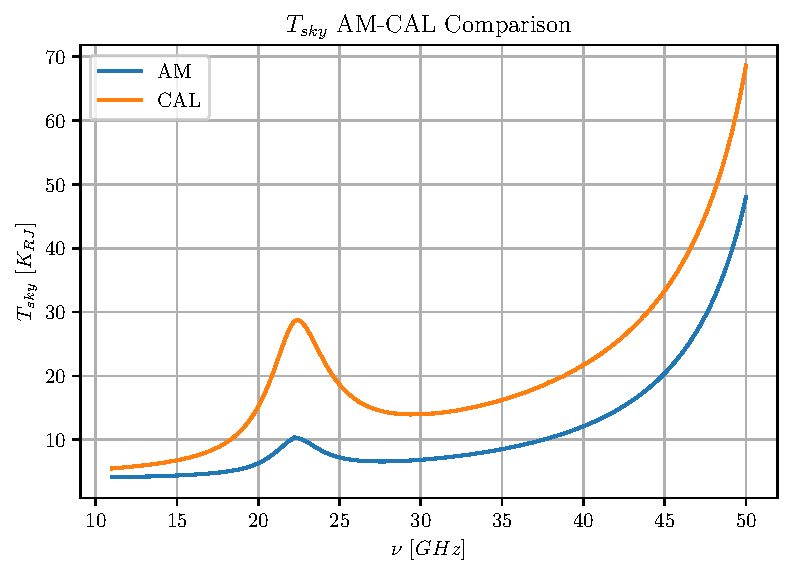
\includegraphics[width=\textwidth]{AM_CAL_Comparison}
        \caption{AM/CAL sky brightness temperatures comparison.}
        \label{fig:am_cal_comparison}
\end{figure}

\begin{figure}
        \centering
        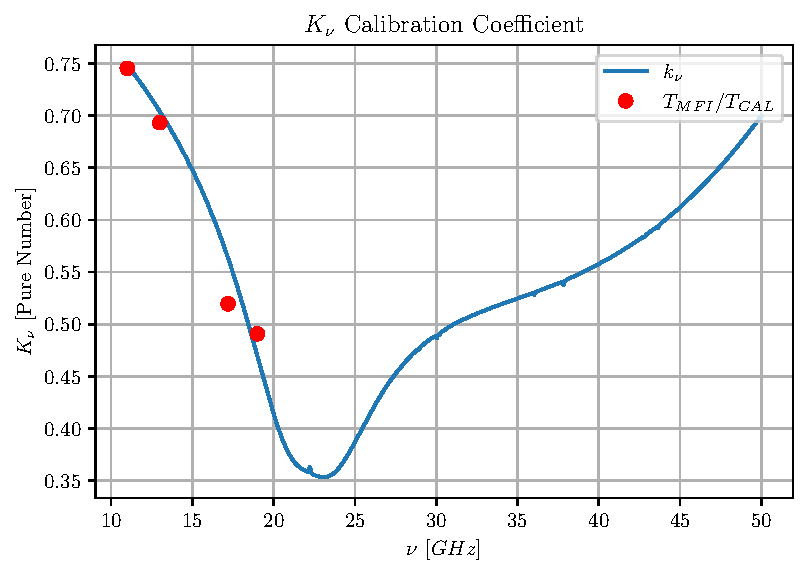
\includegraphics[width=\textwidth]{Calibration_Coefficient_QUIJOTE}
        \caption{$K_\nu$ calibration coefficient.}
        \label{fig:calibration_coefficient_quijote}
\end{figure}

\section{Comparison with Calibrated Data}

\begin{figure}
        \centering
        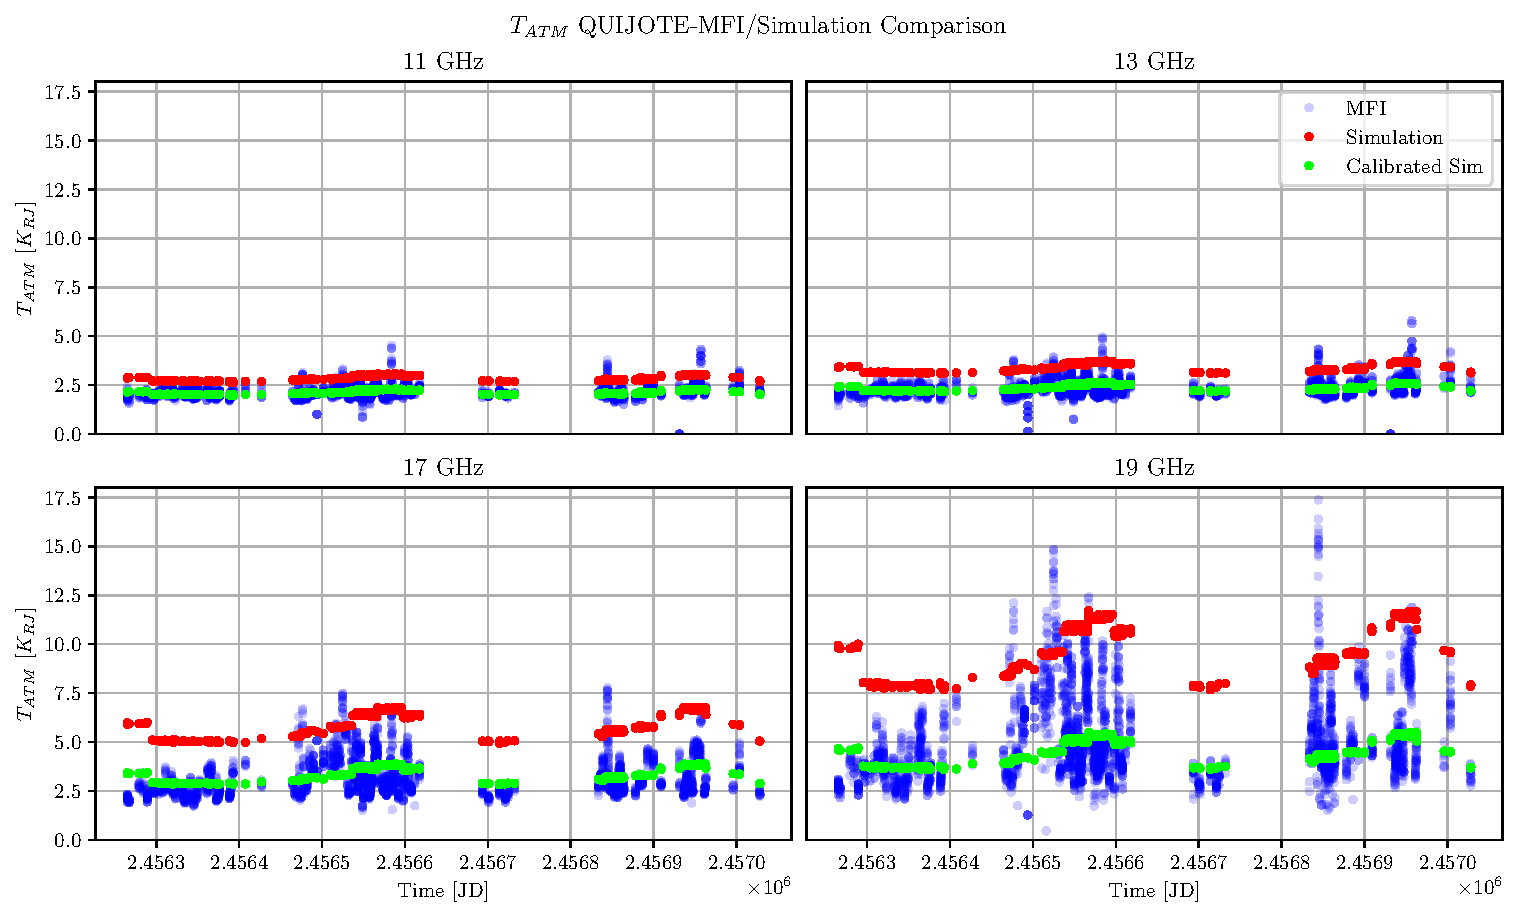
\includegraphics[width=\textwidth]{QUIJOTE-Sim_calibrated}
        \caption{Comparison between QUIJOTE-MFI measurements and
        CAL simulated data with calibration applied.}
        \label{fig:quijote_sim_calibrated}
\end{figure}

